\chapter{Software Architecture Design}
In this chapter, we will discuss the process of software architecture design. It is a crucial step of software engineering. It is so important because a poor architecture might often result in low quality, reliability and maintainability. It also makes development more difficult. The architecture is hard to developed in an incremental way, and is costly to change in the later stages. Therefore, enough attention should be paid to the architecture design.

\section{Layered Software Architecture}
There are different types of software architectures, such as layered architecture, event-driven architecture, micro-kernel architecture, micro-services architecture, cloud architecture etc. The layered architecture is the most widely used, and the de facto standard software architecture. (ref: software architecture patterns).

The layered architecture contains roughly four layers: the presentation layer, the business layer, the persistence layer, and the database layer. The presentation layer is where the users interact with the software. It displays internal status of the software and receives user inputs. In case of a GUI software, the presentation layer consists of GUI widgets. The business layer is where a certain business logic is defined. The persistence layer, also known as data layer, is where the user access the database layer. The database connector API, for example, is on this layer. The bottom layer is the database layer containing SQL databases, files, and so on.

Each layer contains multiple modules that achieve a specific purpose. Within a specific layer, modules are fairly independent of each other. For example, the system block dialog and the register dialog basically have nothing to do with each other. However, in practice, modules in a certain layer might also need to directly interact with the non-neighboring layers. A well-designed layered architecture allows users to easily revise a certain module, or add a new module into a certain layer, without much modification on other modules on the same layer or neighboring layers.

\section{Layered Architecture Design}
We decided to use the layered software architecture. The architecture basically has four layers, although it can be extended if necessary. With this architecture, what we need to do is divide the software into function modules and fill them into those layers. To design a good layered architecture, it is crucial to define good modules. We have to ask ourselves these questions:
\begin{itemize}
\item What modules should there be?
\item What is the boundary of each function module?
\end{itemize}

We found it might be a good idea to define modules by functionality. For each functionality, we create a UI module and a business logic module. We put them in the presentation layer and business layer respectively. The persistence layer and the database layer in our case is quite straightforward. Intuitively, user authentication shall be somewhere between the presentation layer and the business layer. When users do something on the GUI, the authenticator shall check whether the operation is legal, and determine whether to execute the corresponding business logic function or prompt an error message to the user. In fact, we also want the presentation layer to change its appearance according to the authentication. As a result, we decided we should modify the default 4-layered architecture by adding an authentication layer between the presentation and the business layer.

Following what is discussed, we listed functionalities from the requirements. For many of those functionalities a certain UI component is required. Some functionalities might share a single UI component. For example, when we add or edit a system block, we need the same system block dialog. Finally, we designed the software architecture as below. Only part of the modules are included in the figure.

\begin{figure}[htbp]
\centering
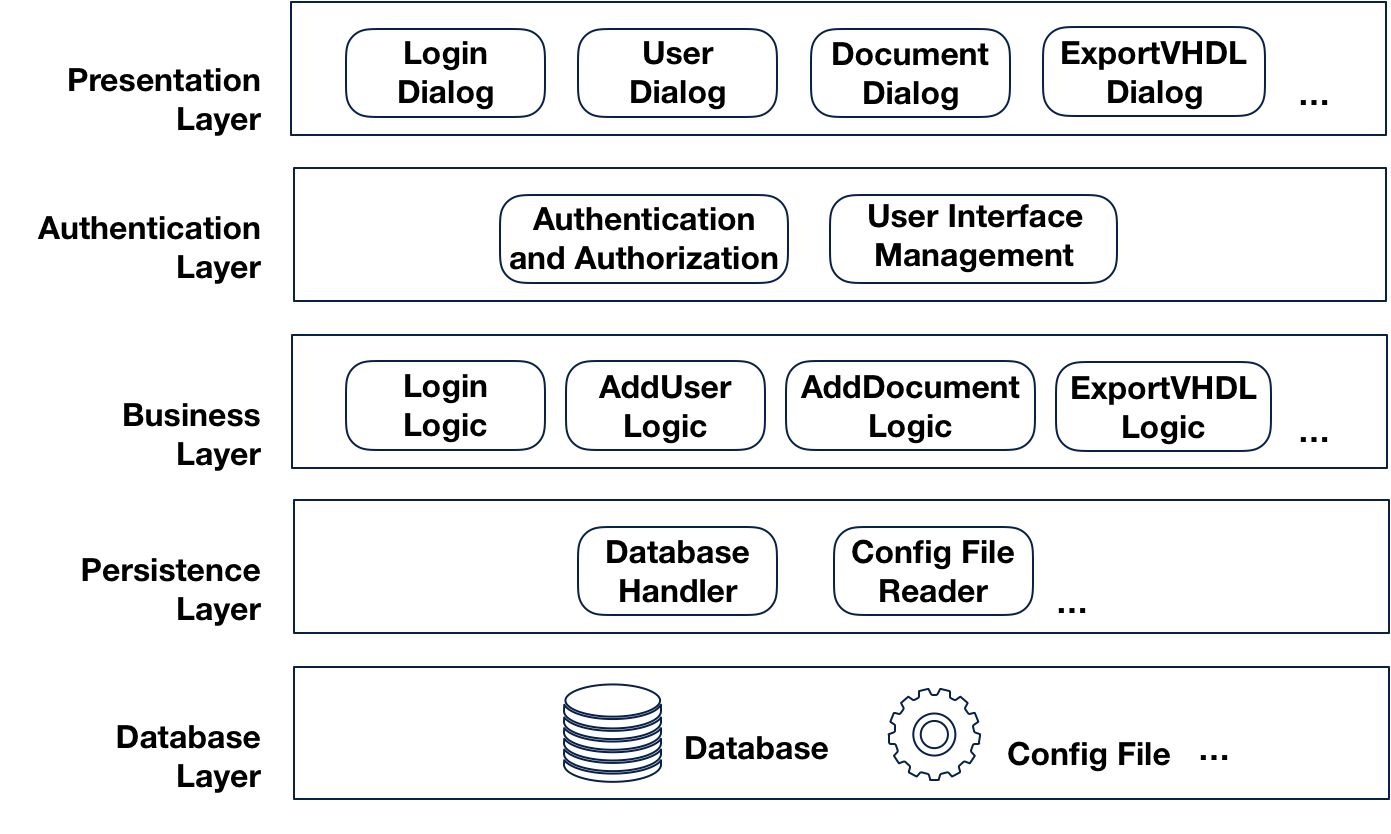
\includegraphics[width = \textwidth]{LayeredArchitecture}
\caption{Layered Architecture\label{fig:Layered Architecture}}
\end{figure}

\section{Object-Oriented System Design}
So far we designed the layered architecture of the software by dividing it into functional modules, and assigning each module to a certain layer. The layered architecture, however, does not model the interactions between modules within a layer or across layers. Also, the models are not associated with any implementation form. In practice, they can be implemented with a class or a function. In this section, we will design the software system in more details following the object-oriented programming paradigm, and finally produce a class diagram. However, at this point we do not consider module module design and implementation details. We will leave this to the next chapter.

\subsection{Object-Oriented Programming}
Object-oriented programming (OOP) is a programming paradigm based on objects. An object contains data and methods. Objects interact with each other and this usually leads to modification of the data in the objects. In the class-based OOP languages, an object is an instance of a class, a template for creating objects and providing initial values and behaviors. 

OOP has three central ideas (Java book)
\begin{itemize}
\item Encapsulation: the classes hide their internal status, and only expose necessary information. Another important idea is inheritance.
\item Inheritance: it represents the "is-a-type-of" relationship between classes.
\item Polymorphism: it provides a single interface to entities of different types.
\end{itemize}

The definition of classes and their relationships can be represented by the UML class diagram. The class is represented with a rectangle with three boxes. The top box contains the class name. The members variables (i.e. the data) are in the middle box. In the bottom box are member methods. The member variables and methods are decorated with +, \# or - representing public, protected and private respectively. Classes related to others are connected with lines of different forms. Relationships can be categorized into instance-level and class-level. According to the degree of dependency, instance-level relationships are dependency, association, aggregation and composition. Dependency relationship exists when an instance references another. Association represents a "has-a" relationship. Aggregation and composition are variants of the "has-a" association relationship in that they represent a "is-part-of" relationship. The difference is, the composition relationship entails ownership. If class A has a composition relationship with B, when B is destroyed A will be destroyed too. The class-level relationships reflect the inheritance relationships between classes. The two relationships differ in that realization involves an abstract superclass, aka an interface. 

\begin{figure}[htbp]
\centering
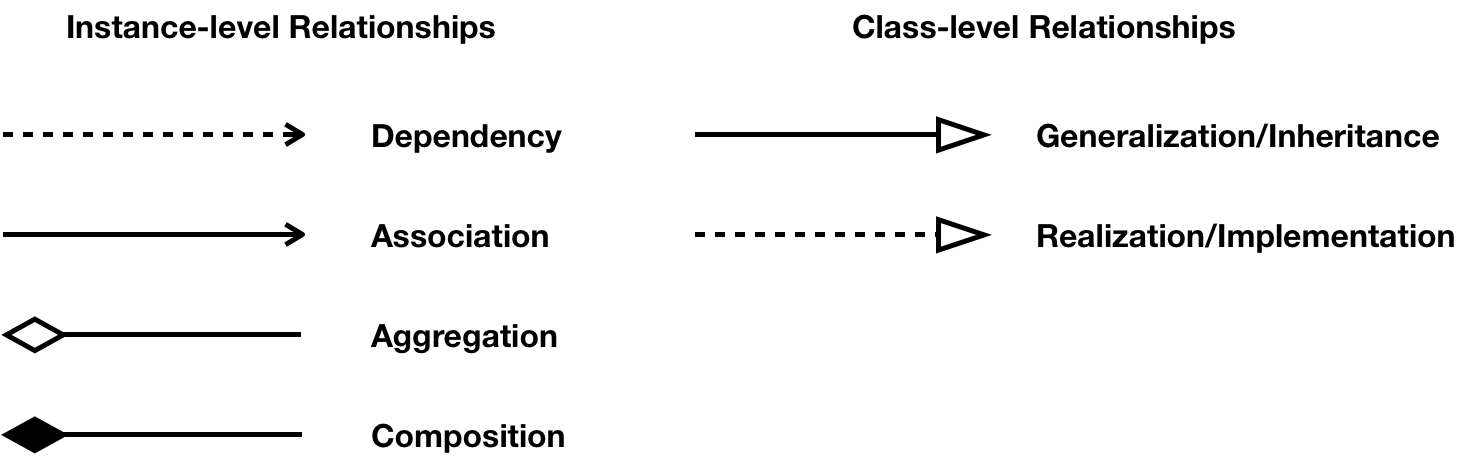
\includegraphics[width = \textwidth]{ClassRelationships}
\caption{Class Relationships\label{fig:Class Relationships}}
\end{figure}

\subsection{System Design}
With the OOP background, our task is to design the system and produce a class diagram.  At this point, we have to answer two questions
\begin{itemize}
\item What classes should there be and what they do?
\item What are their relationships with each other?
\end{itemize}
These two questions are not independent. The answer to one can influence the other.

In Qt, a general design pattern is to first design a UI form using the Qt Creator, and then design the class incorporating the UI as one of its member variable. We can design the UI in a WYSIWYG manner. The Qt Creator will then generate a UI form in XML format containing all information about the UI, and a C++ class from the UI form. Then, we will create a class with an instance of the UI class. We can then write business logic functions in this class. In this way, modules in the presentation layer and business logic layers are unified. 

Some functionalities require user input. For example, to add a system block the name, abbreviation and start address of the system block must be given by the user. The client requires developers to design an appropriate dialog for such use cases. However, the dialog can be reused for different functionalities. The system dialog can be used for not only adding but also editing system blocks, for example. In such cases, a single UI class can be associated with multiple functionalities. Following the same pattern, we can design dialog classes for other functionalities such as adding or editing a signal, register and so on. Since these functionalities are independent of each other, these classes basically do not have relationships with each other, and we can design and implement them in an incremental manner.

According to the requirements, the main window shall contain a chip navigator, a chip editor view and a document editor view. Intuitively, we can design a ChipNavigator, ChipEditorView and DocumentEditorView class respectively. The ChipEditorView displays information about the chip and provides access to those functional dialogs related to chip editing. Similarly, the DocumentEditorView displays documentations and provides access to document editing dialogs. The MainWindow itself is also associated with global level functional dialogs such as SPIGenerationDialog, DocumentationGenerationDialog, ChangePasswordDialog and so on. In the end, the system can be illustrated with the class diagram below.

\begin{figure}[htbp]
\centering
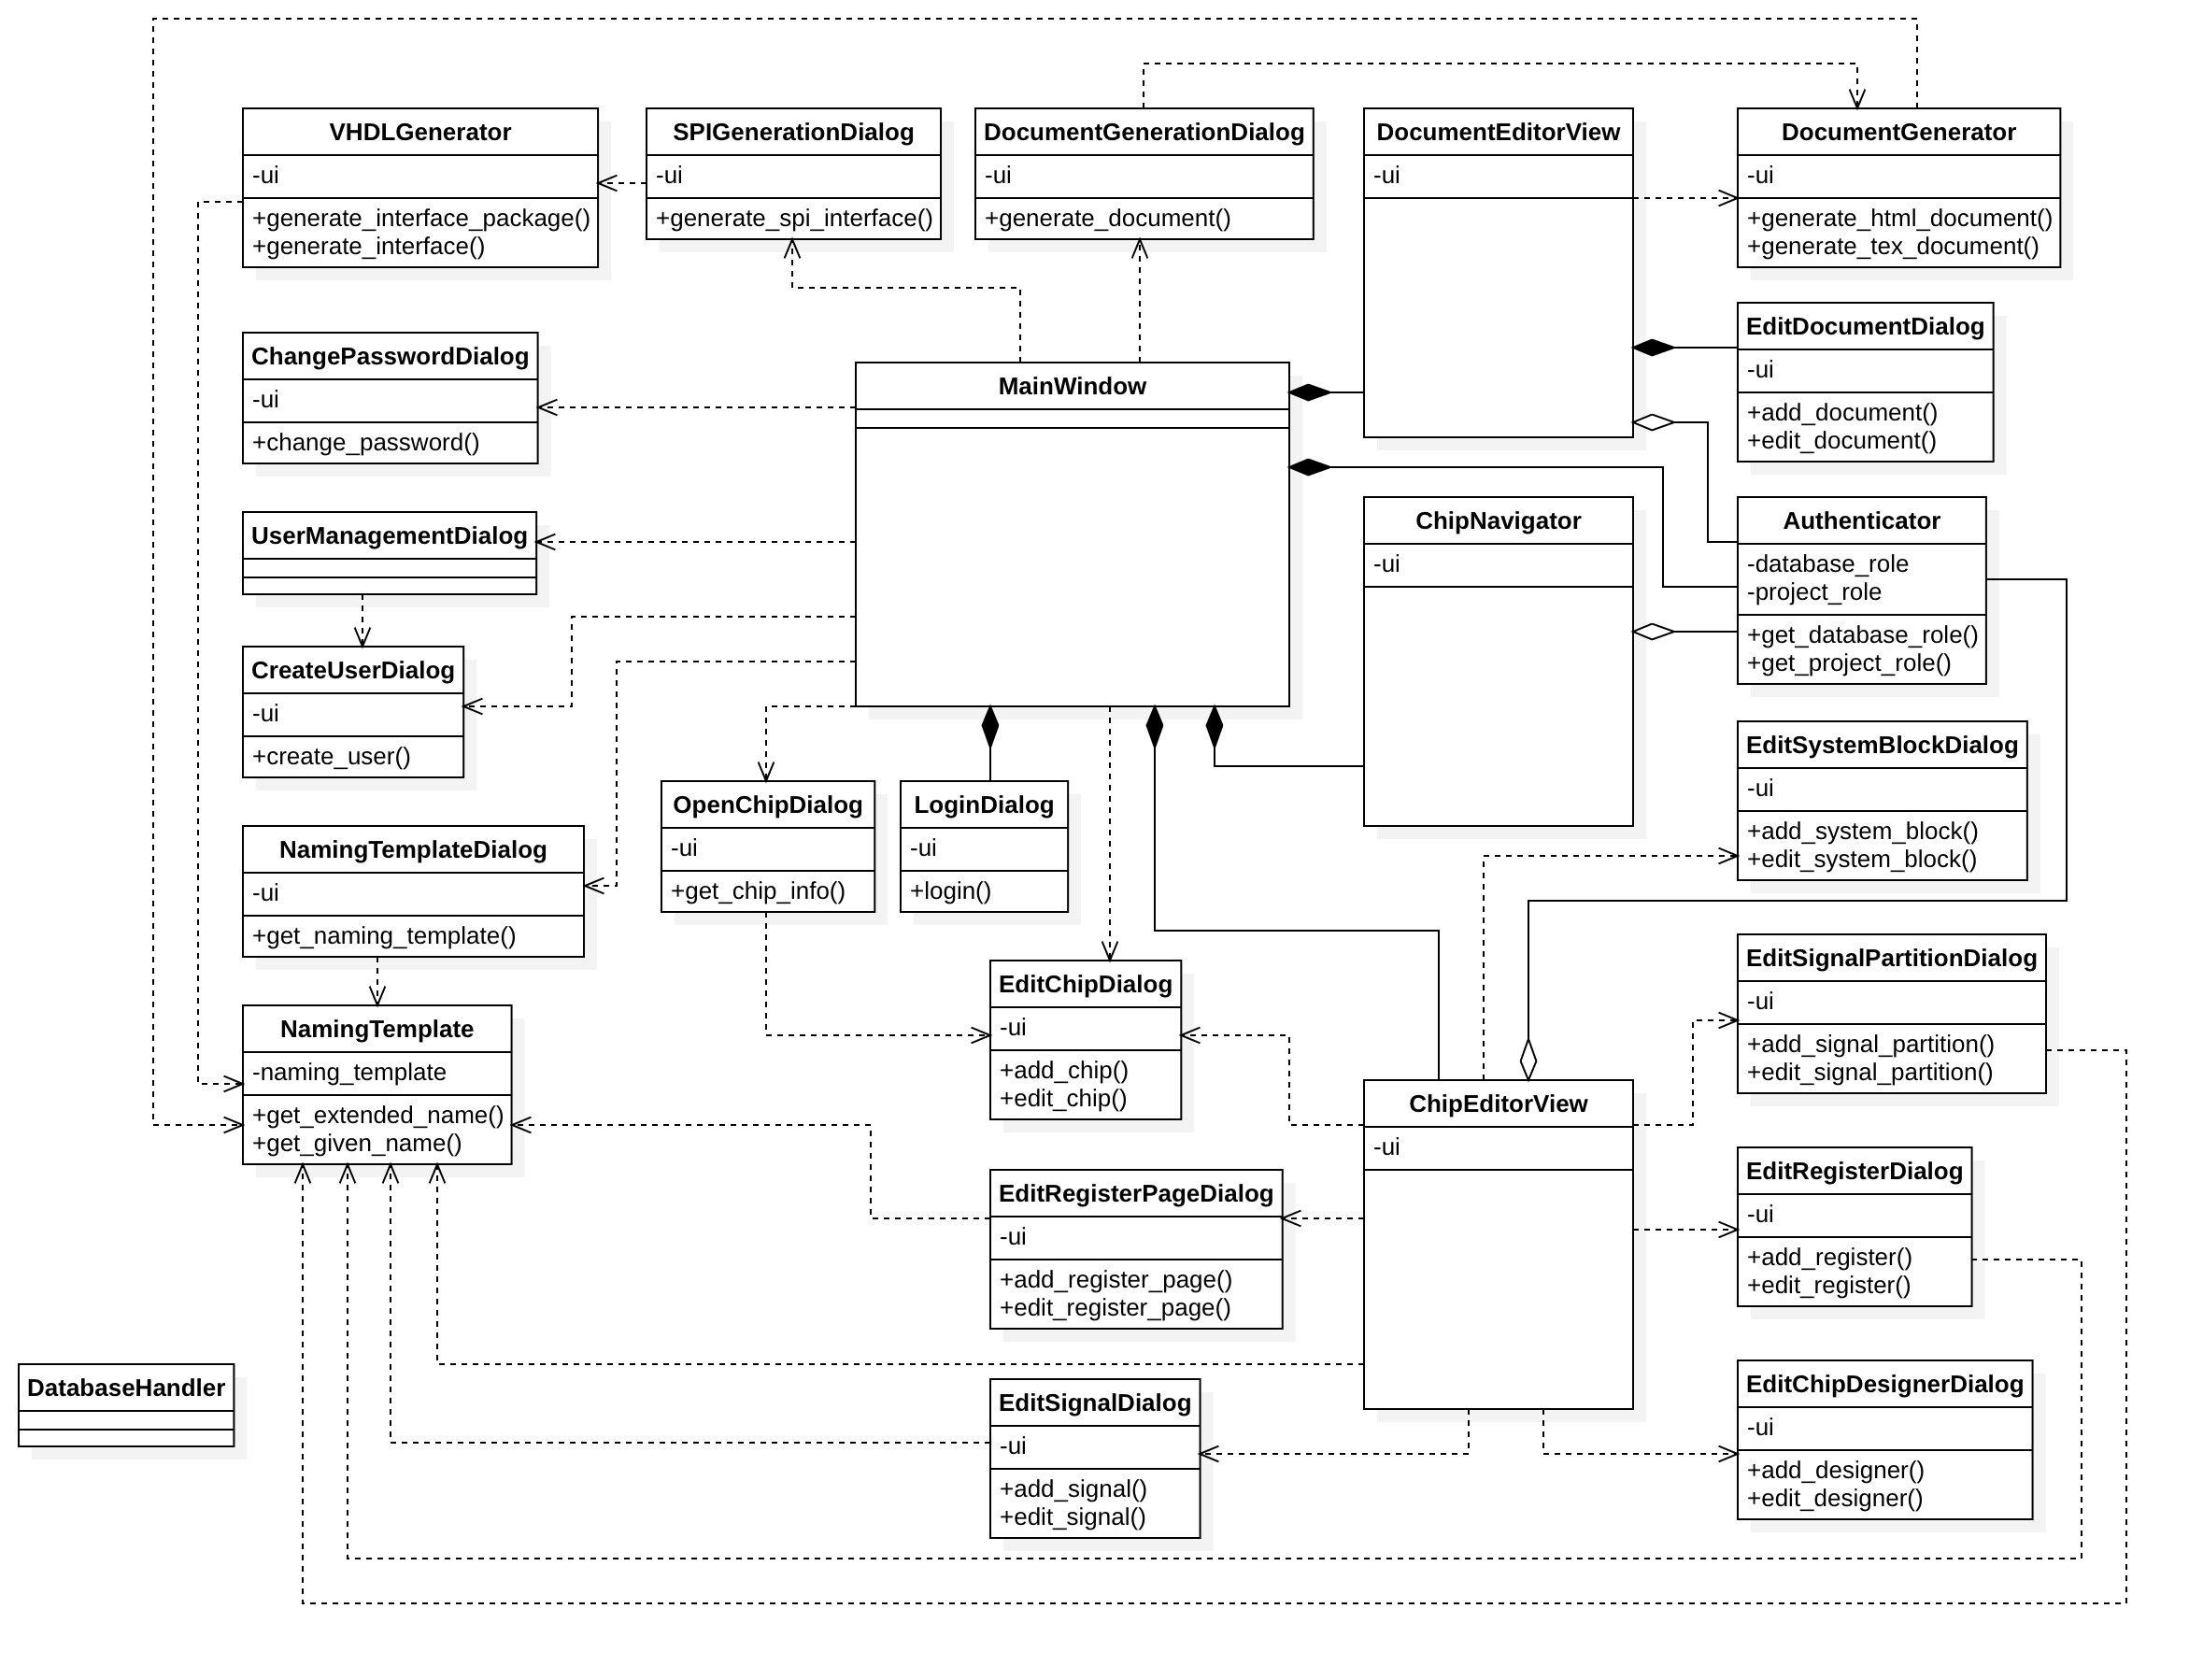
\includegraphics[width = \textwidth]{RegisterManagerClassDiagram}
\caption{Register Manager Class Diagram\label{fig:Register Manager Class Diagram}}
\end{figure}

Note that this class diagram is simplified in many ways. First, it only shows classes we want to create. The classes provided by Qt are omitted. The UI classes are not in the diagram either. Instead, they appear as a member named "ui" of many classes in the diagram. Since we are still in the design phase so the classes are incomplete. Only the most important member variables and methods are shown in the diagram. Also, most classes have dependency relationship with the DatabaseHandler class. However, their relationships are omitted in the diagram so as to make the diagram more readable and understandable.

The center of the software is the MainWindow. From the diagram we see that the MainWindow \textbf{has} a ChipNavigator, ChipEditorView, DocumentEditor, Authenticator and a LoginDialog. Unlike other Dialog classes such as CreateUserDialog, the LoginDialog is a member of the class MainWindow and it exits in the whole lifetime of the software (which is exactly the lifetime of the MainWindow). This is because we consider that users may want to log out and log in with another account. The MainWindow are directly dependent of many dialogs which are not directly associated to the DocumentEditorView or the ChipEditorView. These dialogs are not members of the class MainWindow. When they are needed, a certain action is triggered by the user and a temporary instance will be created.

The ChipNavigator, ChipEditorView and DocumentEditorView are members of the MainWindow and they exist in the whole life cycle of the software. The ChipEditorView are dependent of those chip editor dialogs including EditChipDialog, EditSystemBlockDialog, EditRegisterDialog. The DocumentEditorView is dependent of the DocumentGenerator. Likewise, these dialogs are created only when needed.

A special case is the Authenticator. It is the major component of the authentication layer. It stores the database permissions and project permissions of the current user to the current project. Whenever the current status changes, for example, when the user clicks on another system block on the navigator, permissions are requested and the UI are updated by enabling or disabling certain widgets. The MainWindow has a member Authenticator. The pointer to the member Authenticator is passed to the ChipNavigator, ChipEditorView and DocumentEditorView, such that they actually access the same Authenticator instance.

Dependency relationships between the MainWindow, ChipEditorView etc to the functional dialogs are easy and clear because those functional dialogs are basically independent of each other. However, the relationships between the ChipNavigator to the ChipEditorView and DocumentEditorView are tricky. In our design, they are not directly related to each other, but via the MainWindow. Whenever the user clicks on something in the navigator, it will "tell" the MainWindow that something is triggered by sending it a signal (will be discussed in the next chapter). The MainWindow then updates the current system block, register, signal etc, and updates the status of the ChipEditorView and DocumentEditorView by function calls. Likewise, when the chip is edited, the ChipEditorView sends a signal to the MainWindow. The MainWindow then calls a corresponding function to update the navigator.

To generate the SPI interface and the documentation, we use the SPIGenerationDialog and the DocumentGenerationDialog. With these dialogs, we can specify necessary input and configure the output. The DocumentGenerationDialog then creates a DocumentGenerator and calls the corresponding methods to create documentation rather in LaTeX or HTML format. To generate the SPI interface, the DocumentGenerationDialog creates a certain type of generator given the format of the output. For example, to generate VHDL code, the dialog creates a VHDL generator.

The NamingTemplate is designed in response to the requirement that the names of registers and signals shall be formatted. For example, we may want all register names to start with the block abbreviation and end with "REG". To set up a naming template, we use the NamingTemplateDialog.

Although the class diagram does not regard how each class works, but only what they do, we cannot design a system completely without considering the design and implementation details of each class. We will discuss this in the next chapter.